\subsubsection*{Fairness methods}
Another question fair machine learning deals with is how algorithms can be adjusted so that they fulfil one of the above fairness metrics.
Depending on when they take place in the machine learning pipeline, we distinguish between
\begin{enumerate}
    \item Pre-processing methods
    \item In-processing methods
    \item Post-processing methods
\end{enumerate}
Pre-processing methods follow the idea that the data should be modified before training, so that the algorithm learns on "corrected" data. Reweighing observations before training is an example for a preprocessing method. The idea is to assign different weights to the observations based on relative frequencies, so that the algorithm learns on a balanced dataset \cite{caton2024}.\\
In-Processing methods modify the optimization criterion, such that it also accounts for a chosen fairness metric. Introducing a regularization term to the loss function is one example of such modifications.\\
Post-processing methods work with black box algorithms, just like preprocessing methods. We only need the predictions from the model to adjust them so that again a chosen fairness metric is fulfilled. One example for this is thresholding, where we set group specific thresholds to re-classify the data after training (\cite{hardt2016}).
Depending on the task (regression, classification) and the model there are highly specified and advanced methods. For the case study in chapter 3, we limit ourselves to methods from the \texttt{mlr3fairness} package.
% mlr3fairness currently has two preprocessing methods, one postprocessing method and several fairness adjusted models implemented. We decide to use a reweighing methods that works with assigning weights to the observations to equalise the distribution of $P(Y|PA)$.
% The inprocessing method is a fairness-adjusted logistic regression implemented in mlr3fairness inspired by Zafar et. al. This method optimises for statistical parity (independence). The postprocessing method we choose aims for equalised odds and it works by randomly flipping a subset of predictions with pre-computed probabilities in order to satisfy equalised odds constraints.

\subsubsection*{Bias and the feedback loop}
\begin{figure}
    \centering
    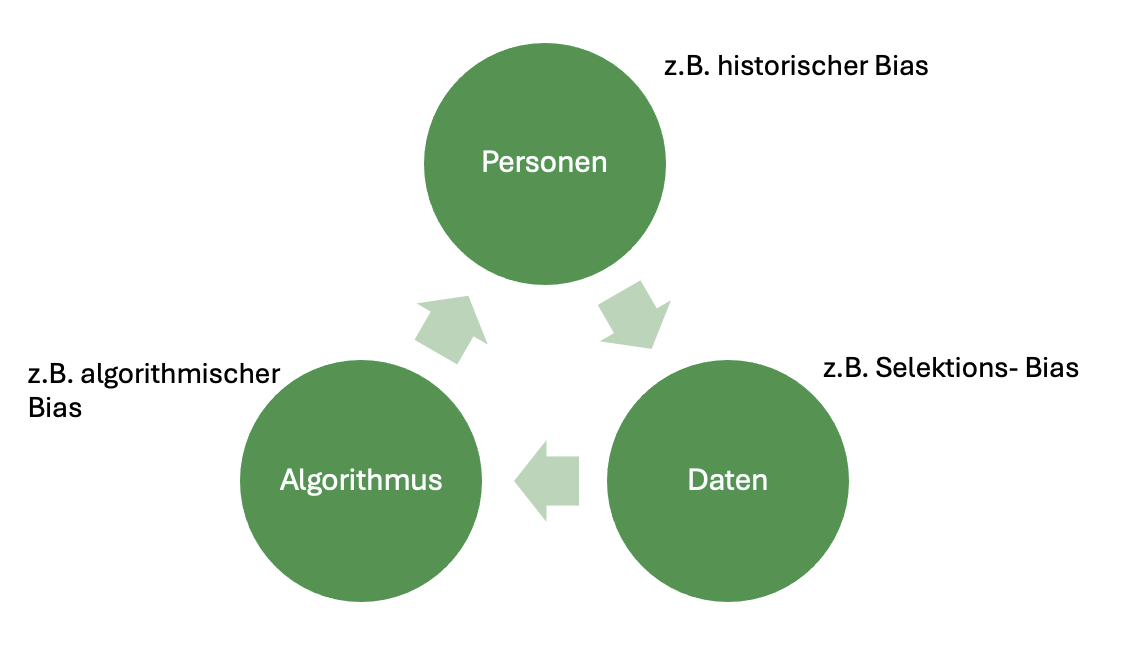
\includegraphics[width=0.7\textwidth]{../figures/bias_loop.png}
    \caption{The bias loop.}
    \label{fig:bias_loop}
\end{figure}

Before the application on real data, to introduce different types of biases and the context in which the ADM is embedded.
Used to assist decision-making, the machine learning model influences if someone gets admitted to college, receives a loan or is released from prison. This means the algorithm does not exist in isolation, but is embedded in a loop with data and the user.\\
The circumstances of a decision are made measurable by collecting data. The algorithm learns from this data to make an optimal prediction, on which the decision-makers base their judgement on \autoref{fig:bias_loop}. At each step of this loop, bias can be introduced in the process and, more dangerous, be amplified as the algorithm influences decision-making on a large scale.
This means that every fairness project comes with the task to understand where the data comes from and how exactly the algorithm will be deployed in practice.\\
Depending on at which station of the user, algorithm, feedback loop bias is introduced into the process, different types of bias can be distinguished. We refer to x for an extensive overview of the different types of bias. It can be crucial to think about which type of bias might be relevant in a given situation as this should influence the definition of fairness and the choice of fairness adjustments. This will also become clear in the context of SQF.\\

% \subsection*{Bias}
% We want to end this general introduction into fair machine learning by outlining the context in which the algorithm is usually embedded. On this note we also advice practitioners to think about the source of bias that could be present in your situation, as this \textit{should} influence how fairness is defined and what fairness adjustments are appropriate. This will motivate the potential difficulties that can arise when implementing fairness in the real world.
% \cite{caton2024} describe the situation as follows. The algorithm is embedded in a feedback loop with the user and data.
% We as a society make decision, which reflect our reality. We make our reality measurable by collecting data. The algorithm learns from this data and makes predictions, on which we base new decisions. 
% At each of these three points bias can be introduced into the process and, above all, bias can also be reinforced in the course of this process.
% In the context of the Stop, Question, and Frisk data, historical bias and selection bias are probably the most relevant sources of bias.
% Historical bias can shows itself in different ways. In our case it would mean that we assume that some people in our data have repeatedly experienced discrimination in terms of being arrested.
% Selection bias refers to the fact that the data is not representative of the population of New York City, because the decision to stop someone is based on a biased decision policy.



